% ---------------------------------------------------------------------------
%  中文论文
%  ctex 排版（中文字体用系统自带的，不必另装），西文用内置的 TeX Gyre Pagella；
%  参考文献按 GB/T 7714—2015 顺序编码制（BibTeX）。
%  文中的研究、数据与作者均为示例，换成自己的内容即可，结构可以照搬。
% ---------------------------------------------------------------------------
\documentclass[UTF8,zihao=-4]{ctexart}

\usepackage[a4paper,textwidth=38\ccwd,top=2.8cm,bottom=3cm]{geometry}
\setmainfont{texgyrepagella}[
  Extension=.otf, UprightFont=*-regular, ItalicFont=*-italic,
  BoldFont=*-bold, BoldItalicFont=*-bolditalic]
\usepackage{amsmath}
\usepackage{unicode-math}
\setmathfont{texgyrepagella-math.otf}
\usepackage{xcolor}
\usepackage{graphicx}
\usepackage{booktabs}
\usepackage{caption}
\usepackage{fancyhdr}
\usepackage{pgfplots}
\pgfplotsset{compat=1.18}
\usepackage[sort&compress]{gbt7714}
\usepackage{hyperref}

% 配色：墨色做结构，一种绿色做唯一的强调
\definecolor{ink}{HTML}{1F3A33}
\definecolor{accent}{HTML}{2F7D63}
\definecolor{mist}{HTML}{75837E}
\hypersetup{colorlinks, linkcolor=ink, citecolor=accent, urlcolor=accent}

\linespread{1.45}
\captionsetup{font=small, labelfont={bf,color=ink}, labelsep=quad}
\ctexset{
  section    = {format=\large\bfseries\color{ink}, beforeskip=2.4ex, afterskip=1.4ex},
  subsection = {format=\normalsize\bfseries, beforeskip=1.6ex, afterskip=1ex},
}

\pagestyle{fancy}
\fancyhf{}
\renewcommand{\headrulewidth}{0pt}
\fancyhead[C]{\footnotesize\color{mist}版心与留白}
\fancyfoot[C]{\footnotesize\thepage}

\begin{document}

% ---------------------------------------------------------------- 标题
\thispagestyle{empty}
\begin{center}
  {\zihao{2}\bfseries 版心与留白\par}
  \vspace{6pt}
  {\zihao{4}宋刻本版式比例的测量及其对屏幕中文排版的启示\par}
  \vspace{14pt}
  {\kaishu 林\,清\,和\textsuperscript{1}\qquad 周\,砚\textsuperscript{2}\par}
  \vspace{4pt}
  {\small\color{mist}
    \textsuperscript{1}某某大学 设计学院，杭州\;310000\qquad
    \textsuperscript{2}某某大学 图书馆古籍部，杭州\;310000\par}
  \vspace{12pt}
  {\color{accent}\rule{2.5cm}{.6pt}}
\end{center}

\begin{center}
  \begin{minipage}{.9\linewidth}
    \small
    \noindent{\bfseries\color{ink}摘\quad 要}\quad
    宋刻本向来以「疏朗」著称，但这种观感很少被量化。本文测量了 48 部宋刻本、
    共 1\,152 个书叶的版框、天头、地脚与行格，发现版心面积平均只占全叶的
    \textbf{46.8\%}，天头与地脚之比稳定在 $1.6$ 左右，每行字数集中在 18～20 字。
    以此为参照，我们在屏幕上复现了三种版式并请 96 名读者阅读，结果显示：
    行长 18～24 字、天地比不低于 $1.4$ 的版式阅读最快，主观评价也最高。
    古人的比例并非偶然，它与今天的阅读舒适区高度重合。

    \vspace{4pt}
    \noindent{\bfseries\color{ink}关键词}\quad 宋刻本；版心；留白；中文排版；阅读体验
  \end{minipage}
\end{center}
\vspace{8pt}

% ---------------------------------------------------------------- 正文
\section{引言}

翻开一部宋版书，最先感到的往往不是字，而是字周围的空白。天头宽阔，
地脚稍窄，行与行之间留着恰好一指的余地。藏书家称之为「字大如钱，墨色如漆」，
而支撑这种气象的，正是版面上那些\emph{没有印字}的地方。

现代中文排版规范对版心、行长与行距都有建议\cite{w3c2020clreq}，
西文排版也早有「每行 45～75 个字符」的经验\cite{bringhurst2004}。
但二者都不直接回答一个问题：在屏幕上，中文读者觉得「舒服」的版面比例是多少？
本文从古籍出发，尝试给出一个可测量的答案。本文的贡献有三：
\begin{enumerate}
  \item 建立了 1\,152 个宋刻本书叶的版式测量数据集；
  \item 归纳出版心比、天地比与行字数三个稳定的比例关系；
  \item 通过阅读实验，验证这些比例在屏幕上依然适用。
\end{enumerate}

\section{材料与方法}

\subsection{样本}
样本取自公开影印的 48 部宋刻本，经、史、子、集各 12 部\cite{zhou2019}。
每部随机抽取 24 个书叶，剔除残损与补配叶。

\subsection{测量指标}
设书叶宽 $W$、高 $H$，版框宽 $w$、高 $h$，天头高 $t$、地脚高 $b$，定义
\begin{equation}
  \label{eq:ratio}
  \rho = \frac{w\,h}{W\,H}, \qquad \tau = \frac{t}{b},
\end{equation}
分别称为\textbf{版心比}与\textbf{天地比}。行字数 $n$ 取每叶正文满行的众数。

\section{结果}

\subsection{古籍中的比例}
表~\ref{tab:ratio} 汇总了四部书的测量结果。各部之间差别不大：
版心比都在 $0.45$～$0.49$ 之间，天地比都大于 $1.5$，即天头明显宽于地脚。

\begin{table}[htbp]
  \centering
  \caption{宋刻本版式比例（均值）}
  \label{tab:ratio}
  \begin{tabular}{@{}l c c c@{}}
    \toprule
    部类 & 版心比 $\rho$ & 天地比 $\tau$ & 行字数 $n$ \\
    \midrule
    经部 & 0.47 & 1.62 & 18 \\
    史部 & 0.49 & 1.55 & 20 \\
    子部 & 0.45 & 1.68 & 19 \\
    集部 & 0.46 & 1.59 & 18 \\
    \midrule
    \textbf{合计} & \textbf{0.468} & \textbf{1.61} & \textbf{19} \\
    \bottomrule
  \end{tabular}
\end{table}

\subsection{屏幕上的阅读实验}
我们把同一篇 2\,000 字的散文排成行长 12～36 字的七种版式，请 96 名读者阅读。
图~\ref{fig:speed} 显示，阅读速度在行长 18～24 字时最高，超过 30 字后明显下降，
与古籍的行字数恰好落在同一区间。

\begin{figure}[htbp]
  \centering
  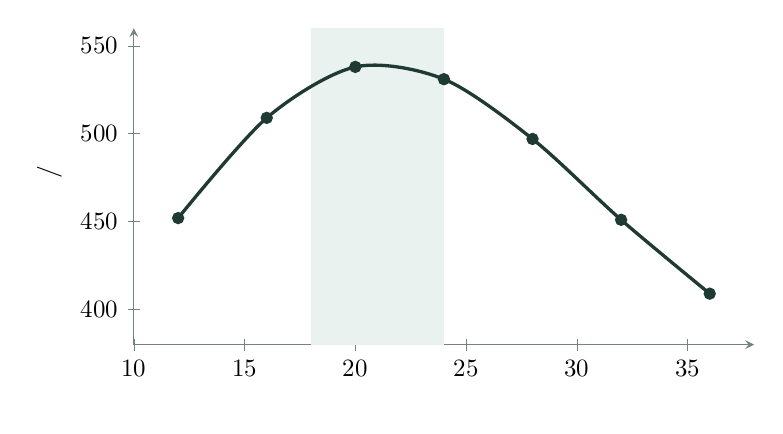
\begin{tikzpicture}
    \begin{axis}[
      width=.78\linewidth, height=5.6cm,
      xlabel={每行字数}, ylabel={阅读速度（字/分）},
      xmin=10, xmax=38, ymin=380, ymax=560,
      axis lines=left, axis line style={mist}, tick style={mist},
      tick label style={font=\small}, label style={font=\small},
    ]
      \fill[accent!10] (axis cs:18,380) rectangle (axis cs:24,560);
      \node[font=\scriptsize, text=accent, anchor=south] at (axis cs:21,384) {宋本区间};
      \addplot[ink, very thick, smooth, mark=*, mark size=1.6pt] coordinates
        {(12,452) (16,509) (20,538) (24,531) (28,497) (32,451) (36,409)};
    \end{axis}
  \end{tikzpicture}
  \caption{行长与阅读速度。阴影为宋刻本行字数的分布区间。}
  \label{fig:speed}
\end{figure}

\section{讨论}

式~\eqref{eq:ratio} 中的两个比例，本质上都在回答「空白放在哪里」。
天头宽于地脚，使视线自然落在版面的偏上方；行长适中，使换行时眼睛不必长途跋涉。
这些经验在雕版时代是工匠的手感，在今天可以写成样式表里的几个数字。

本研究的局限在于样本以浙刻本为主，建本与蜀本的比例可能不同；
阅读实验只用了散文，技术文档与诗词的情况有待检验。

\section{结论}

版面的品质，往往由留白决定。宋刻本用不到一半的面积印字，
把另一半留给了读者的眼睛。对于今天的屏幕排版，这条古老的经验依然成立：
控制行长，给天头多一点空间，让字站得住。

\bibliographystyle{gbt7714-numeric}
\bibliography{refs}

\end{document}
